\documentclass{article}
%Preamble
\usepackage{float}
\usepackage{color}
\usepackage{listings}
\usepackage{longtable}
\usepackage{amsmath,amssymb}
\usepackage{graphics}
\usepackage{graphicx}

\title{AE 706 -Computational Fluid Dynamics \\ Assignment 1: Report \\ Floating Point Arithmetic}
\author{Aditi Taneja}
\date{}

\begin{document}
\pagenumbering{arabic}
\maketitle

\textbf{1. Write code in C to find the epsilon of the machine for both the float and double types.} 
\\
\newline
Following machine epsilon were obtained for float, double and long double data types.

\begin{figure}[H] \label{figure}
\includegraphics[width=12cm]{one.png}
\caption{Epsilon for Different Data types in C++}
\label{figure:}
\end{figure}

\begin{description}
\item[]Thus, machine epsilon for a data type is equal to $2^{-n}$ where n is length of mantissa for that datatype. ( 23 for float, 52 for double and 64 for long double).
\item[]It can be concluded that Data type for temporaries in C++ is double, because when no data type is allocated to 0.5, it's data type becomes double and when multiplied by (float data type) epsilon makes it double ( larger size data type).
\item[]However, when double 0.5 is multiplied with long double epsilon, result is in long double data type for the same reason as above.
\end{description}

\textbf{Q2:Write code in Python or your favorite language (octave, scilab etc.) to find the epsilon of the machine.}

\begin{figure}[H] \label{figure}
\includegraphics[width=12cm]{two.png}
\caption{Machine epsilon for float data types in python}
\label{figure:}
\end{figure}
\begin{description}
\item[]'float' data type in python is equivalent(same in size) to double in C++.
\item[]'numpy.float128' data type in python is equivalent(same in size) to long double in C++. 
\end{description}

\textbf{Q3:Plot the function
$f(x)=\frac{(1 − cos(x))}{x^2}$
\\
in the region $[-4e-8 <= x <= 4e-8]$ using your favorite programming language. Plot the correct curve and show how you obtain it.}
\newline
\begin{figure}[H] \label{figure}
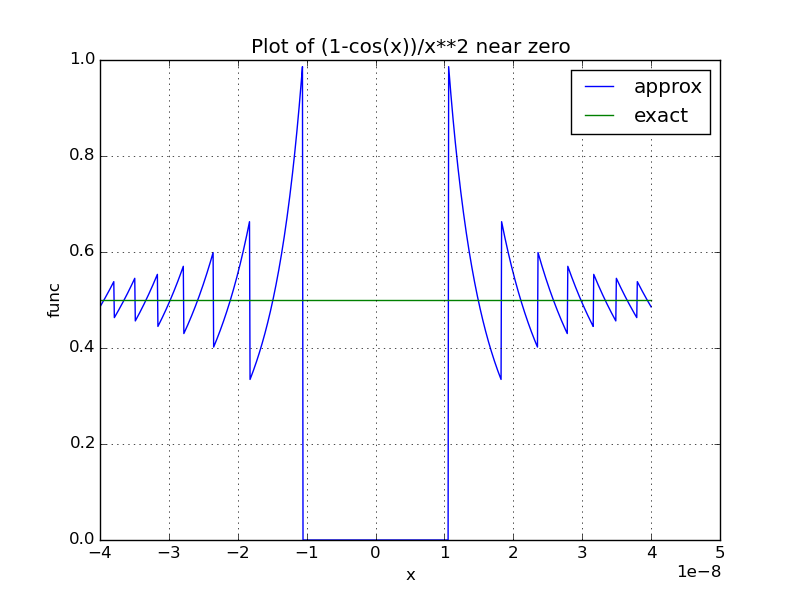
\includegraphics[width=10cm]{three.png}
\caption{Plot with Float(x)}
\label{figure:}
\end{figure}

\begin{figure}[H] \label{figure}
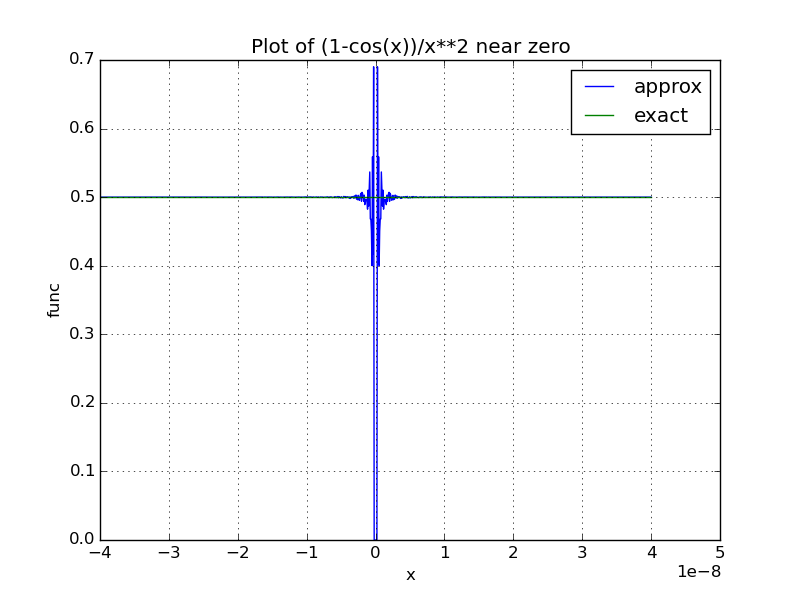
\includegraphics[width=10cm]{three_2.png}
\caption{Plot with Float128(x)}
\label{figure:}
\end{figure}

\begin{description}
\item[]As the data type of variable $x$ in the given function is changed from float to float128, the fluctuating region near zero shrinks as shown above. This is because size of mantissa increases and hence precision (length of mantissa is equal to the precision) in the calculations.
\item[]Fluctuation occurs when this function is plotted very close to zero because subtraction is not a well-conditioned arithmetic operation. When $(1-cos(x))$ is calculated very close to zero, $cos(x)$ tends to 1 and hence while calculating (1-cos(x)), huge loss of significant digits occur. This leads to huge relative errors in calculation of $(1-cos(x))$ and hence these fluctations.
\item[]The function value goes to zero when $x$ is very close to zero, while the exact value is 0.5. This happens because value of $cos(x)$ becomes so close to 1 that its floating point approximation becomes equal to 1.0 and hence $(1-cos(x))$ becomes 0.
\item[]Such fluctuations can be avoided by using an alternate function for f(x) so as to avoid subraction between very close numbers. For example: (1-cos(x)) can be written as $\frac{sin^2(x)}{x^2(1+cos(x))}$. Here Taylor series expansion of $cos(x)$ has been used and is been truncated after 50 terms in the expansion of $cos(x)$.
\end{description}

\textbf{Q4. Write out the finite difference form for the first derivative of a $f(x)$ with a first order approximation (forward or backward), second order $(O(h^2))$ and fourth order approximation.}
\begin{description}
\item[] A forward difference approximation for first order derivative is
\\F'(x) = $\frac{F(x + h) − F(x)}{h}+ O(h)$
\item[]A backward difference approximation for first order derivative is
\\F'(x) = $\frac{F(x) − F(x-h)}{h}+ O(h)$
\item[]A centered difference approximation ($ O(h^2)$) for first order derivative is
\\F'(x) = $\frac{F(x + h) − F(x-h)}{2h}+ O(h^2)$
\item[]A centered difference approximation ($ O(h^4)$) for first order derivative is
\\F'(x) = $\frac{−F(x + 2h) + 8F(x + h) − 8F(x − h) + F(x − 2h)}{12h}+ O(h^4)$
\end{description}
\textbf{Q5. Consider f(x) = sin(x) at the point x=pi/4.  Start with h=pi/4, compute the value of the first derivative for each scheme.  Keep halving h and compute the relative error between the computed value of the derivative and the exact value as you successively halve h.  Plot this on a log-log scale.}

\begin{figure}[H] \label{figure}
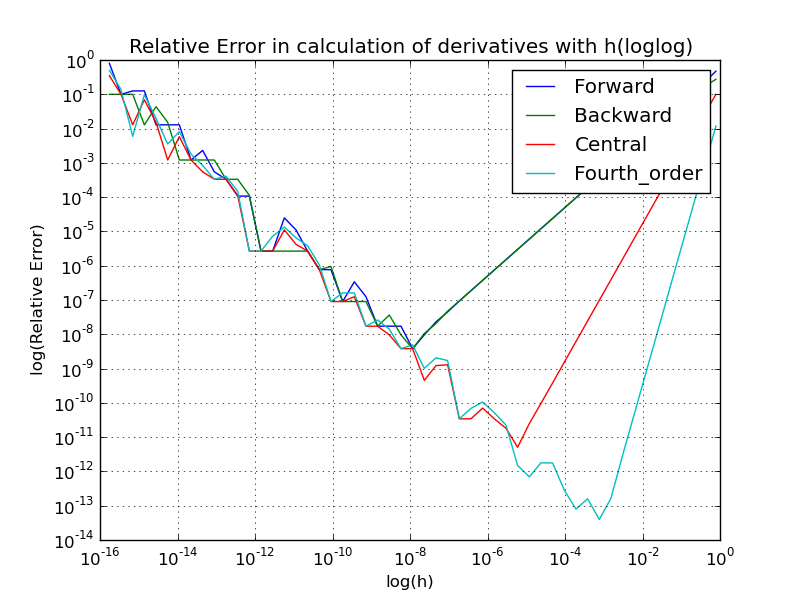
\includegraphics[width=10cm]{five.png}
\caption{Relative Error in calculation of derivatives with h(loglog)}
\label{figure:}
\end{figure}
\begin{description}
\item[] The order of error can be seen from the slope of plots obtained for relative error in approximation of first order derivative with order1 (Slope = 1), 2(Slope = 2) and 4(Slope = 4). 
\item[] As h is decreased, relative error in the approximation of first order derivatives decreases at different slopes (equal to the order of the error) till some point but then increases at almost same slope. 
This happens because as h is decreased, $f(x+h) or f(x-h)$ become more close to $x$, and hence the approximate value becomes closer to the exact value of the derivative of the function and hence error decreases. 
However, when h is decreased below a certain value, $f(x+h) or f(x-h)$ become so close to $f(x)$ that the subtraction operation between them leads to loss of significant digits and as h becomes smaller and smaller, error is amplified since h comes in the denominator.

\item[] Fluctuations start at higher h for $4^{th}$ order, then $2^{nd}$ order, and then $1^{st}$ order because as the order of error increases, the approximate value converges faster to the exact value and hence loss of significant digits while subtracting become significant at earlier stage (higher h).  
\end{description}


\end{document}
